\PassOptionsToPackage{unicode=true}{hyperref} % options for packages loaded elsewhere
\PassOptionsToPackage{hyphens}{url}
%
\documentclass[man,floatsintext]{apa6}
\usepackage{lmodern}
\usepackage{amssymb,amsmath}
\usepackage{ifxetex,ifluatex}
\usepackage{fixltx2e} % provides \textsubscript
\ifnum 0\ifxetex 1\fi\ifluatex 1\fi=0 % if pdftex
  \usepackage[T1]{fontenc}
  \usepackage[utf8]{inputenc}
  \usepackage{textcomp} % provides euro and other symbols
\else % if luatex or xelatex
  \usepackage{unicode-math}
  \defaultfontfeatures{Ligatures=TeX,Scale=MatchLowercase}
\fi
% use upquote if available, for straight quotes in verbatim environments
\IfFileExists{upquote.sty}{\usepackage{upquote}}{}
% use microtype if available
\IfFileExists{microtype.sty}{%
\usepackage[]{microtype}
\UseMicrotypeSet[protrusion]{basicmath} % disable protrusion for tt fonts
}{}
\IfFileExists{parskip.sty}{%
\usepackage{parskip}
}{% else
\setlength{\parindent}{0pt}
\setlength{\parskip}{6pt plus 2pt minus 1pt}
}
\usepackage{hyperref}
\hypersetup{
            pdftitle={Understanding the impacts of video-guided activities on parent-child interaction},
            pdfauthor={George Kachergis, Emily Hembacher, Veronica Cristiano, Hanwen Vivian Zhang, \& Michael C. Frank},
            pdfkeywords={digital parenting advice; joint attention; lexical diversity; guided play},
            pdfborder={0 0 0},
            breaklinks=true}
\urlstyle{same}  % don't use monospace font for urls
\usepackage{graphicx,grffile}
\makeatletter
\def\maxwidth{\ifdim\Gin@nat@width>\linewidth\linewidth\else\Gin@nat@width\fi}
\def\maxheight{\ifdim\Gin@nat@height>\textheight\textheight\else\Gin@nat@height\fi}
\makeatother
% Scale images if necessary, so that they will not overflow the page
% margins by default, and it is still possible to overwrite the defaults
% using explicit options in \includegraphics[width, height, ...]{}
\setkeys{Gin}{width=\maxwidth,height=\maxheight,keepaspectratio}
\setlength{\emergencystretch}{3em}  % prevent overfull lines
\providecommand{\tightlist}{%
  \setlength{\itemsep}{0pt}\setlength{\parskip}{0pt}}
\setcounter{secnumdepth}{0}
% Redefines (sub)paragraphs to behave more like sections
\ifx\paragraph\undefined\else
\let\oldparagraph\paragraph
\renewcommand{\paragraph}[1]{\oldparagraph{#1}\mbox{}}
\fi
\ifx\subparagraph\undefined\else
\let\oldsubparagraph\subparagraph
\renewcommand{\subparagraph}[1]{\oldsubparagraph{#1}\mbox{}}
\fi

% set default figure placement to htbp
\makeatletter
\def\fps@figure{htbp}
\makeatother

\shorttitle{Impacts of videos on parent-child interaction}
\affiliation{
\vspace{0.5cm}
\textsuperscript{1} Department of Psychology, Stanford University\\\textsuperscript{2} Gallaudet University\\\textsuperscript{3} Cornell University}
\keywords{digital parenting advice; joint attention; lexical diversity; guided play\newline\indent Word count: 4995}
\usepackage{csquotes}
\usepackage{upgreek}
\captionsetup{font=singlespacing,justification=justified}

\usepackage{longtable}
\usepackage{lscape}
\usepackage{multirow}
\usepackage{tabularx}
\usepackage[flushleft]{threeparttable}
\usepackage{threeparttablex}

\newenvironment{lltable}{\begin{landscape}\begin{center}\begin{ThreePartTable}}{\end{ThreePartTable}\end{center}\end{landscape}}

\makeatletter
\newcommand\LastLTentrywidth{1em}
\newlength\longtablewidth
\setlength{\longtablewidth}{1in}
\newcommand{\getlongtablewidth}{\begingroup \ifcsname LT@\roman{LT@tables}\endcsname \global\longtablewidth=0pt \renewcommand{\LT@entry}[2]{\global\advance\longtablewidth by ##2\relax\gdef\LastLTentrywidth{##2}}\@nameuse{LT@\roman{LT@tables}} \fi \endgroup}


\usepackage{lineno}

\linenumbers
\usepackage{float}

\title{Understanding the impacts of video-guided activities on parent-child interaction}
\author{George Kachergis\textsuperscript{1}, Emily Hembacher\textsuperscript{1}, Veronica Cristiano\textsuperscript{2}, Hanwen Vivian Zhang\textsuperscript{3}, \& Michael C. Frank\textsuperscript{1}}
\date{}

\authornote{

Correspondence concerning this article should be addressed to Michael C. Frank, Stanford, CA 94305 USA. E-mail: \href{mailto:mcfrank@stanford.edu}{\nolinkurl{mcfrank@stanford.edu}}}

\abstract{
Early parenting practices play an important role in shaping the future outcomes of young children (Hart \& Risley, 1995; Heckman, 2006).
In particular, high-quality early interactions and language input appear to facilitate language learning and result in higher levels of school performance.
The rise of phone- and tablet-based parenting applications (``apps'') holds the promise of delivering low-cost, positive interventions on parenting style to a wide variety of populations.
Of special interest are the parents of very young children, who are often difficult to reach in other ways. Yet little is known about the effects of communicating to parents through app-based interventions.
We showed parents a short video depicting an age-appropriate parent-child activity from a commercial parenting app, and found that the quality of parent-child interactions increases in some ways as a result of the intervention.
Specifically, after watching the activity video, parents spoke more and made more bids for joint attention with the child.


}

\begin{document}
\maketitle

\hypertarget{introduction}{%
\section{Introduction}\label{introduction}}

The quantity and quality of early language input has been found to be strongly associated with later language and academic outcomes (Cartmill et al., 2013; Hart \& Risley, 1995; Hirsh-Pasek et al., 2015; Marchman \& Fernald, 2008; see Schwab \& Lew-Williams, 2016 for a review). Thus, because of the potential for large downstream effects (Heckman, 2006), there is tremendous interest in interventions that change children's language environment.
And because parents define a large portion of that environment, especially before the onset of formal schooling, parent behavior is a critical locus for such interventions.
Many effective parenting interventions require large resource investments and require many hours of in-person contact (Gertler et al., 2014; Leung, Hernandez, \& Suskind, 2018; Schweinhart et al., 2004), making implementation at scale a daunting proposition.
For this reason, many researchers targeting early language are interested in delivering parenting interventions remotely -- through texts, apps, and videos delivered on digital devices.
But what do parents take away from these short messages about what to do with or how to talk with their children?

The content provided by digital parenting interventions runs the gamut from general parenting messages and facts from child development research to specific advice and suggested activities.
A growing body of evidence suggests that these digital interventions can be effective across a range of cultures, income levels, and children's ages (for a review, see Breitenstein, Gross, \& Christophersen, 2014).
For example, in contrast to a face-to-face parent training intervention, a tablet-based version saw significantly higher session completion rates (51\% attendance vs.~85\% module completion) and comparable or larger effect sizes on parents' and children's (aged 2 to 5 years) behavior (Breitenstein, Fogg, Ocampo, Acosta, \& Gross, 2016).
Often, however, the theory of change presupposed by such interventions is relatively vague.
Both within and outside the realm of academic interventions, messages to parents of young children often seek to provide knowledge about some aspect of development (e.g., early language), often in tandem with a suggestion regarding activities.
Such messages are assumed to inform parents' choice of behaviors, spurring them to engage in some target activity, which is assumed to be more stimulating than what parents would have done otherwise.

This theory of change is typically grounded in ideas about guided play and early language stimulation.
Child-directed speech varies not only in quantity (i.e., the number of total tokens), but also in quality in terms of the diversity of the tokens (Malvern, Richards, Chipere, \& Durán, 2004) or the context-appropriateness of the speech (Cartmill et al., 2013), both of which have been linked to children's subsequent language development.
Further, language learning---especially the acquisition of early vocabulary in the first years---appears to be supported preferentially by parents and children \emph{jointly attending} to some object or activity (Baldwin, 1991; Bigelow, MacLean, \& Proctor, 2004).
Episodes of joint attention are frequent during guided play, when parents set goals and scaffold their child's activities (Weisberg, Hirsh-Pasek, \& Golinkoff, 2013; Wood, Bruner, \& Ross, 1976).
Thus, the current literature supports interventions that encourage parents to provide high-quality language and interaction through something like guided play---whether via reading books or playing with a shape-sorter at home, or via a conversation about categories in the supermarket.

But is this theory of change correct? That is, does the provision of knowledge and activities lead to higher-quality play?
Alternatively, by focusing parents on a specific activity, this approach could be flawed, causing parents to over-focus on achieving the superficial goals of the activity.
This problem might be especially likely with video messages, which could encourage parents to try to mimic a model's specific speech and/or actions.
Attempting to reproduce such surface details of a video-guided activity could in turn result in less high-quality talk, with less responsiveness to their child's play.
Another possibility is that these messages might produce the desired effect, but only for those parents who already have a general orientation towards children's early learning.

Our current experiments were designed to make a direct test of this question: How do parents change their interactions with young children on the basis of short video parenting messages?
In two experiments, we collected data from parent-child dyads in a local children's museum.
We showed parents in the experimental group a single short video modeling an interactive toy-based activity along with a scientific justification.
Parents in the control group received either no video (Experiment 1) or a video of a recent finding in developmental psychology (Experiment 2).
We then gave the toys from the video to all dyads and videotaped their interactions, coding for caregivers' language quantity and quality as well as joint attention.

\hypertarget{experiment-1}{%
\section{Experiment 1}\label{experiment-1}}

In Experiment 1, we invited parents of 6- to 24-month-old infants visiting the Children's Discovery Museum in San Jose to complete video-guided activities from a commerical parenting app that delivers digital parenting advice in the form of short videos.
Parents were randomly assigned to one of two conditions: parents in the \emph{Activity Video} condition watched a video from the app (matched to their child's age), and then performed the activity with their child using the props from the video.
Parents in the \emph{No Video} condition did not watch an activity video, but were given a set of the same age-appropriate props and asked to play with their infants as they normally would at home.

\hypertarget{method}{%
\subsection{Method}\label{method}}

\hypertarget{participants.}{%
\subsubsection{Participants.}\label{participants.}}

60 infants (F = 43, M = 17) aged 6-24 months (19 6-11.9 month-olds: 9 in the control condition, 10 in Activity Video; 20 12-17.9 month-olds: 11 control, 9 Activity Video; 21 18-24 month-olds: 10 control, 11 Activity Video) and their parents participated in a museum in northern California.
We included infants who were exposed to English at least 50 percent of the time (n = 58) or who were exposed less but whose participating parent reported that they primarily speak English with their child at home (n = 2).
62\% of participants (n = 37) had been exposed to two or more languages, as indicated by their parent.
Parents identified their children as White (n = 25), Asian (n = 11), African American/Black (n = 2), Biracial (n = 12), other (n = 5), or declined to state (n = 5).
Fifteen parents reported that their child was of Hispanic origin.
Parents tended to be highly-educated, with reports of highest level of education ranging from completed high school (n = 5), some college (n = 7), four-year college (n = 16), some graduate school (n = 2), to completed graduate school (n = 30).

\hypertarget{materials.}{%
\subsubsection{Materials.}\label{materials.}}

Stimuli included activity videos from a commercial parenting application.
The videos were designed to show activities to parents that they could perform with their child in order to foster cognitive and physical development, and were targeted to the child's age and level of development.
In each video, an adult and child perform the activity (e.g., sorting toys according to size) while a narrator explains the activity and its purpose.
We selected two videos for each of three age groups in our sample (6-11.9 months, 12-17.9 months, 18-23.94 months).
Participants were also given a set of toys corresponding to those in the video that they watched so that they could complete the activity.\footnote{Details of the specific videos used and the toys associated with each video are in the Appendix.}

Participants were randomly assigned to either the \emph{Activity Video} condition or the \emph{No Video} condition.
Parents participating in the Activity Video condition were assigned to watch one of the two activity videos available for their child's age group, while parents in the No Video condition watched no video, and were simply asked to play with their child as they normally would.
The two conditions were yoked: for each Activity Video participant who saw a particular video and received the associated props, a participant in the No Video condition received the same props to use without seeing the video.
Parents also completed the Early Parenting Attitudes Questionnaire (EPAQ; Hembacher \& Frank, 2020).
The EPAQ measures parents of young children's attitudes about parenting and child development along three dimensions: rules and respect, early learning, and affection and attachment (see SI).

\hypertarget{procedure.}{%
\subsubsection{Procedure.}\label{procedure.}}

After providing informed consent, parents in the Activity Video condition watched the assigned activity video on a laptop with headphones.
To ensure that parents could give the video their full attention, the experimenter played with the infant with a set of toys (different from the experimental props used in the study) while the video was being played.
Immediately following the video, each parent-child dyad was provided with the props to complete the video-guided activity that the parent had viewed.
The toys were placed on a large foam play mat, and parents were instructed to sit on the mat with their child and re-create the activity they had viewed for a period of approximately three minutes.\footnote{Based on piloting, we estimated these activities would would only require three minutes to complete.}
In the No Video condition, after informed consent parents were told to play with their child as they would at home with the provided props for a period of three minutes.
They were not given any additional instructions about how to use the props.

In both conditions, two video cameras were used to record the play session from different angles, and parents were fitted with a wireless Shure lavalier microphone to record their child-directed speech.
After three minutes of play had elapsed, parents were told they could stop playing and the cameras and microphone were turned off.
Parents were then asked to complete the EPAQ before being debriefed.

\hypertarget{joint-attention-coding-procedure.}{%
\subsubsection{Joint Attention Coding Procedure.}\label{joint-attention-coding-procedure.}}

The video of each session was manually coded for episodes of joint attention (JA) using the Datavyu software (Team, 2014).
The video taken at floor level was coded by default, but the other video was referred to if the participants were occluded or if there was technical difficulty with the first camera.
Each session's video was coded for episodes of coordinated JA, episodes of passive JA, and parental bids for JA.
Parental bids for JA were defined as any attempt to initiate joint attention (i.e labeling, pointing, or otherwise drawing attention to an object) that did not result in passive or coordinated JA.
If more than 3 seconds elapsed between bids, they were coded as separate attempts.
An episode of joint attention was considered \emph{passive} if both participants visually focused on an object for 3 or more seconds but the child did not acknowledge the parent.
If either participant looked away from the object for less than 3 seconds and then returned to the same object it was considered part of the same episode of joint attention.
A joint attention episode was considered \emph{coordinated} if both participants visually focused on an object for 3 or more seconds and at some point in the interaction the child indicated awareness of interaction with some overt behavior toward the parent such as looking at their face, gesturing, vocalizing, or turn-taking.
Full details of our guidelines for coding joint attention are available in SI.

A second coder independently coded a third of the videos (i.e., 20 of the 60 videos, approximately equally distributed across ages) to establish reliability.
The two coders had a reliability of ICC = 0.79 with 95\% confidence interval (CI) = {[}0.55, 0.91{]} for rate of parent bids for JA (number of bids per minute); ICC = 0.34 with 95\% CI = {[}-0.11, 0.67{]} for rate of passive JA episodes (per minute); ICC = 0.66 with 95\% CI = {[}0.32, 0.85{]} for rate of coordinated JA episodes; ICC = 0.33 with 95\% CI = {[}-0.11, 0.67{]} for time spent (seconds per minute) in passive JA episodes, and ICC = 0.60 with 95\% CI = {[}0.24, 0.82{]} for time spent in coordinated JA episodes.

\hypertarget{results-and-discussion}{%
\subsection{Results and Discussion}\label{results-and-discussion}}

Parents' child-directed speech during the play sessions (mean duration: 3.25 min) was transcribed; child utterances were not considered.
Although Experiment 1 was not preregistered, for consistency the transcripts and hand-coded joint attention data were analyzed according to our preregistration for Experiment 2\footnote{Preregistration: \href{https://osf.io/2bpdf}{https://osf.io/2bpdf/}}, with any deviations or exploratory analyses noted.
Below we first report the lexical diversity results, followed by the joint attention results.

\hypertarget{lexical-diversity}{%
\subsubsection{Lexical Diversity}\label{lexical-diversity}}

For each transcript of child-directed speech, the caregivers' unique word \emph{types} and \emph{tokens} (total words) uttered were tallied and converted to rates (e.g., tokens per minute of play), and the type-token ratio (TTR) was calculated as a measure of lexical diversity.
Although we initially preregistered TTR as our measure of lexical diversity (since it is a simple, commonly used measure), it has been noted that TTR is correlated with the length of a text, which has led to the development of new measures such as the measure of textual lexical diversity (MTLD; McCarthy \& Jarvis, 2010).
Thus, we also measure lexical diversity with MTLD, which is calculated as the mean length of sequential word strings in a text that maintain a given TTR value (we use 0.72, as proposed by McCarthy \& Jarvis).

We fit a Bayesian mixed-effects linear regression predicting TTR as a function of condition, age (centered), and their interaction with a random intercept per video using rstanarm (Goodrich, Gabry, Ali, \& Brilleman, 2018).
For effects that are at least 95\% likely to be non-zero according to the posterior distribution (i.e., probability of direction: \emph{pd}; Makowski et al. (2019a)), we report estimated coefficients (\(\beta\)) as well as 89\% Bayesian credible intervals (89\% CI)\footnote{89\% CIs are recommended for Bayesian analyses because unless the effective sample size (ESS) is on the order of 10,000, the 95\% credible interval is unstable (Kruschke, 2014; Makowski et al., 2019b; McElreath, 2018). Our ESS ranges from 2,000-5,000, and thus we report the tighter, more stable interval.}, demarcating the range within which 89\% of the posterior falls, meaning that given the observed data, the effect has 89\% probability of falling within this range (see Appendix for more an illustrated explanation).
There was lower TTR in the Activity Video condition (mean: 0.32) than in the No Video condition (mean: 0.43, \(\beta=\)-0.11, 89\% CI = {[}-0.15, -0.07{]}, \emph{pd} = 1).
A similar regression instead predicting MTLD also found lower lexical diversity in the Activity Video condition (mean MTLD: 17.87) than in the No Video condition (mean: 27.09, \(\beta=\)-9.24, 89\% CI = {[}-14.07, -4.21{]}, \emph{pd} = 1), with no notable influence of age.
Figure \ref{fig:lexdiv} (top) shows the mean of each lexical diversity measure (TTR and MTLD) by condition.

We also conducted similar regressions predicting the rate of word tokens and types per minute of play, finding a notable effect of condition on the rate of word tokens (\(\beta=\) 16.50, 89\% CI = {[}5.78, 27.2{]}, \emph{pd} = 0.99), with parents using tokens at a higher rate in the Activity Video condition (mean: 69 tokens/min, bootstrapped 95\% confidence interval (conf. int.): {[}60, 79{]}) than in the No Video condition (mean: 52, 95\% conf. int.: {[}44, 61{]}).

\begin{figure}[H]

{\centering 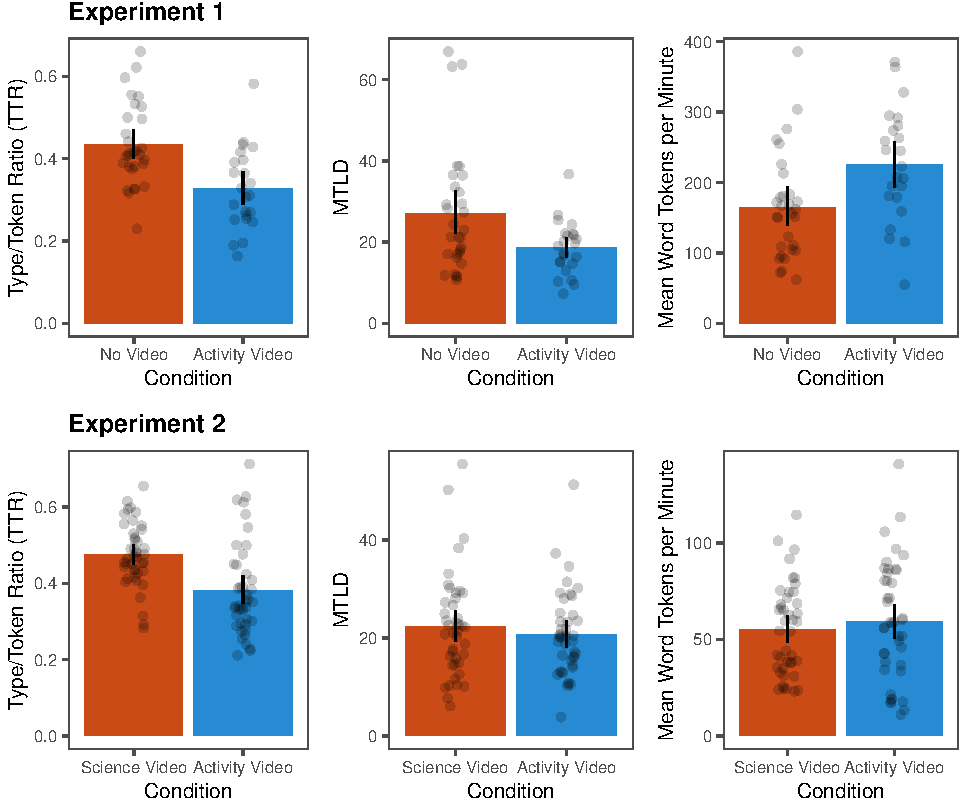
\includegraphics{figs/fig-lexdiv-1} 

}

\caption{\label{fig:lexdiv} Mean lexical diversity scores (left: Type/Token ratio, middle: MTLD) and mean number of tokens used by condition (right) in Experiment 1 (top) and Experiment 2 (bottom). Error bars show bootstrapped 95\% confidence intervals, and gray dots indicate values for each participant.}\label{fig:fig-lexdiv}
\end{figure}

\hypertarget{joint-attention}{%
\subsubsection{Joint Attention}\label{joint-attention}}

We fit a Bayesian mixed-effects linear regression predicting the rate of parent bids (per minute) for joint attention (JA) as a function of fixed effects of condition, age (centered), and their interaction, with random intercepts per video.
Parents' bid rate was greater in the Activity Video condition (mean: 3, sd: 1.11) than in the No Video condition (mean: 2.15, sd: 1.02, \(\beta=0.72\), 89\% CI = {[}0.12, 1.32{]}, \emph{pd} = 0.97).
Mixed-effects regressions with the same structure were performed predicting the rate of episodes of coordinated and passive JA, and the time spent in coordinated and passive JA.
There were no notable effects on the rate of episodes nor on the time spent in coordinated or passive JA episodes.
Figure \ref{fig:JA} (top) shows the mean rate of bids and episodes of JA by condition in Experiment 1.

\hypertarget{exploratory-analyses}{%
\subsubsection{Exploratory Analyses}\label{exploratory-analyses}}

We also fit Bayesian mixed-effects linear regression models predicting each of the above lexical diversity and joint attention dependent variables as a function of fixed effects of condition, age (centered), the child's sex, parent's education level, and the subscales of the EPAQ: Early Learning (EL), Affection and Attachment (AA), and Rules and Respect (RR), along with interactions of condition and EL, AA, and RR.
These models included random intercepts per video.
Of these exploratory regressions, two showed notable effects involving the EPAQ subscales, and one other showed an effect of the child's sex.
First, in the word types regression, parents with higher Affection and Attachment scores used more word types per minute after watching an Activity Video (interaction of condition and AA: \(\beta=6.81\), 89\% CI = {[}0.87, 13.13{]}, \emph{pd} = 0.97).
Second, in the regression examining the rate of passive JA episodes, parents scoring higher on the Rules and Respect (RR) subscale had a lower rate of passive JA episodes (\(\beta=-0.34\), 89\% CI = {[}-0.62, -0.07{]}, \emph{pd} = 0.98).
However, after an Activity Video, higher RR parents did not show this decrease in passive JA (interaction of condition and RR: \(\beta=0.63\), 89\% CI = {[}0.23, 1.03{]}, \emph{pd} = 0.99).
Parents with higher education also showed a lower rate of passive JA episodes (\(\beta=-0.25\), 89\% CI = {[}-0.45, -0.04{]}, \emph{pd} = 0.97).
Finally, parents with male children made bids for JA at a higher rate (mean: 2.76 bids/min) than those with female children (mean: 2.49, \(\beta=0.82\), 89\% CI = {[}0.06, 1.54{]}, \emph{pd} = 0.96).

To get a better sense of the intervention's effect on language use, we analyzed which words were characteristic of parents' speech in each condition, comparing the difference in frequency rank of each word (lemma) in the two conditions, as well as contrasting the corpus overall with a general English-language word frequency list (see SI for the interactive corpus characteristic plot).
Words that were strongly indicative of being from the Activity Video condition include \enquote{give}, \enquote{big}, \enquote{small}, \enquote{ribbit}, \enquote{thank}, \enquote{have}, and \enquote{bus}, while words that were most characteristic of the No Video condition include \enquote{shake}, \enquote{ready}, \enquote{oh}, \enquote{on}, \enquote{going}, \enquote{going}, \enquote{see}, \enquote{let}, and the child's name.

\begin{figure}[H]

{\centering 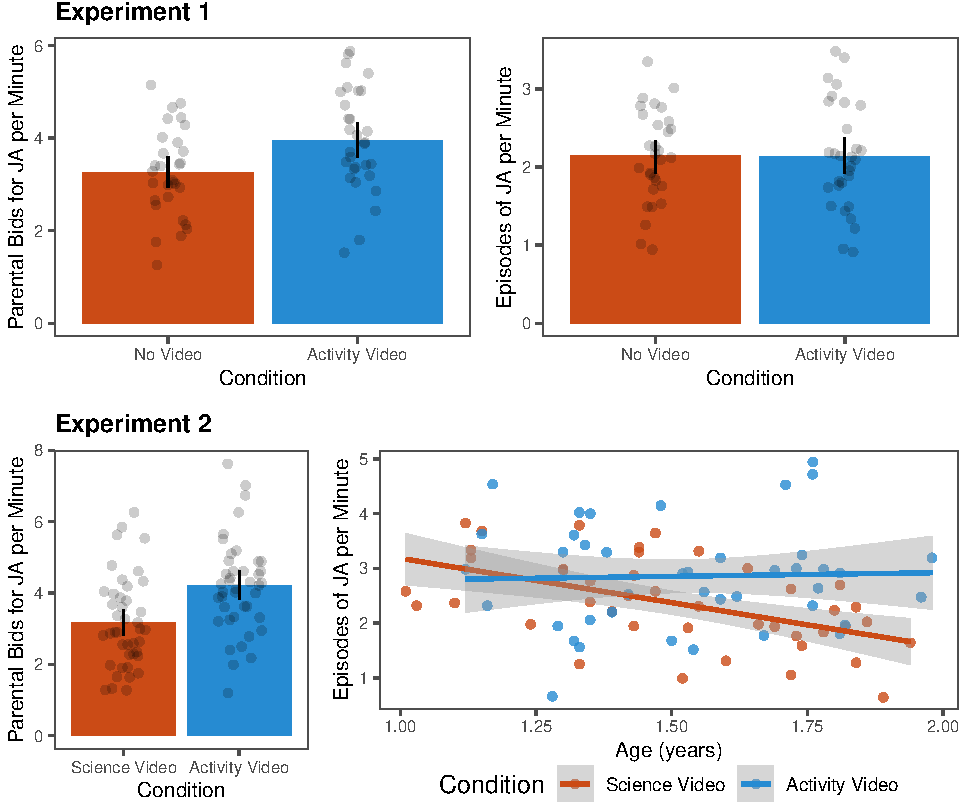
\includegraphics{figs/fig-JA-1} 

}

\caption{\label{fig:JA} Mean number of bids (left) and episodes (right) of joint attention (JA) by condition in Experiment 1 (top). For Experiment 2 (bottom), mean number of bids for JA by condition (left) and the number of episodes of JA by age and condition (right).}\label{fig:fig-JA}
\end{figure}

\hypertarget{discussion}{%
\subsubsection{Discussion}\label{discussion}}

In summary, while parents produced more word types and tokens after viewing the activity video, lexical diversity (both TTR and MTLD) was higher when parents were just asked to play as they normally would.
It may be that parents in the Activity Video condition, in their attempt to stick to the prescribed task, end up repeating themselves more, and indeed some differences in speech acts were notable:
after the Activity Video, parents used more words related to requests (e.g., \enquote{Can I have X? / Give me X. Thank you!}), whereas after no intervention parents' language related more to invitations (e.g., \enquote{Are you ready?} / \enquote{Let's see.}).
However, parents who watched an activity video also made more bids for JA with their child.
This did not result in a greater number of successful episodes of JA---passive or coordinated---than dyads in the No Video condition, although low reliability in passive JA coding (which led us to refine our JA coding guidelines for Experiment 2) may limit our ability to detect an effect there.
In sum, the results of Experiment 1 suggest that digital parenting advice can increase parents' efforts to engage their child in joint attention, expand the volume if not diversity of their speech, and can shift the type of speech acts towards more requests.

\hypertarget{experiment-2}{%
\section{Experiment 2}\label{experiment-2}}

Experiment 1 found that parents who watched an activity video made more bids for joint attention and spoke more words tokens per minute to their children, but had lower lexical diversity compared to parents who played with their children as they normally would at home.
Might it be that parents who are focused on a specific activity show reduced lexical diversity due to their focus on engaging their child in the activity?
Experiment 2 focuses on replicating the key findings using a stronger control group, as well as a restricted number of preregistered predictions.\footnote{Preregistration: \href{https://osf.io/2bpdf}{https://osf.io/2bpdf/}.}

\hypertarget{method-1}{%
\subsection{Method}\label{method-1}}

\hypertarget{participants.-1}{%
\subsubsection{Participants.}\label{participants.-1}}

84 infants (F = 36, M = 46) aged 12-24 months
(20 12-17.9 month-olds in the Activity Video condition;
21 12-17.9 month-olds in the Science Video condition;
22 18-24 month-olds in the Activity Video condition;
21 18-24 month-olds in the Science Video condition) and their parents participated in the same museum as Experiment 1.
We included infants who were exposed to English at least 75 percent of the time or who were exposed less but whose participating parent reported that they primarily speak English with their child at home.
Forty-nine percent of participants (n = 41) had been exposed to two or more languages as indicated by their parent.
Parents identified their children as White (n = 39), Asian (n = 20), African American/Black (n = 1), Biracial (n = 9), other (n = 7), or declined to state (n = 8).
Sixteen parents reported their child was of Hispanic origin.
Parents tended to be highly-educated, with reports of highest level of education ranging from some college (n = 5), four-year college (n = 28), some graduate school (n = 2), to completed graduate school (n = 36) or declined to state (n = 13).

\hypertarget{materials.-1}{%
\subsubsection{Materials.}\label{materials.-1}}

The design of Experiment 2 was similar to that of Experiment 1, except that instead of seeing no video in the control condition, parents instead watched a video that was generally related to child development research, but did not give any specific instructions about how to interact with infants or children.
This condition was included to control for the possibility that differences in language output and joint attention in Experiment 1 could be due to simply cueing parents to think about infants' learning and cognitive development.
The videos presented in the Control Video condition were media clips (available on YouTube) of developmental psychologists explaining their research interleaved with footage of infants or toddlers engaged in developmental research studies.
Thus, the content of the videos superficially matched those in the Activity Video condition, but did not suggest any particular activities.
The videos were trimmed to approximately match the average video length in the Activity Video condition (close to 90 s).
Details of the videos used in the Activity Video conditions are in the Appendix.

\hypertarget{procedure.-1}{%
\subsubsection{Procedure.}\label{procedure.-1}}

The procedure for Experiment 2 matched that of Experiment 1, except that parents in the Control Video condition watched a control video before the play session.
Consistent with the No-Video control condition in Experiment 1, parents in the Control Video condition were told to play with their child as they would at home, and were not given additional instructions.
The coding procedure also matched that of Experiment 1.
To establish reliability a second coder independently coded 25 of the 84 videos, approximately equally distributed across ages.
The two coders had a reliability of ICC = 0.81 with 95\% confidence interval (CI) = {[}0.62,0.91{]} for number of parent bids for JA; ICC = 0.74 with 95\% CI = {[}0.48, 0.88{]} for number of passive JA episodes; ICC = 0.80 with 95\% CI = {[}0.61, 0.91{]} for number of coordinated JA episodes; ICC = 0.72 with 95\% CI = {[}0.44, 0.86{]} for time spent (secs/min) in passive JA episodes, and ICC = 0.88 with 95\% CI = {[}0.75, 0.94{]} for time spent in coordinated JA episodes.

\hypertarget{results-and-discussion-1}{%
\subsection{Results and Discussion}\label{results-and-discussion-1}}

Parents' child-directed speech during the play sessions (mean duration: 3.08 min) was transcribed and processed, and bids and episodes of joint attention were coded according to the same procedure used in Experiment 1.
We first report preregistered regressions\footnote{Although the preregistration implied the use of standard linear mixed-effects regression through the specification of adopting an alpha level of .005 for statistical significance, the non-convergence of some regressions led us to switch to Bayesian regression. Using a Bayesian analysis has the added benefit of not requiring arbitrary changes to alpha levels to correct for multiple comparisons (Gelman, 2008).} predicting TTR and rate of word tokens, as well as an exploratory regression predicting MTLD.
We then turn to preregistered regressions of parental bids for joint attention and the total number of JA episodes.

\hypertarget{lexical-diversity-1}{%
\subsubsection{Lexical Diversity}\label{lexical-diversity-1}}

We fit a Bayesian mixed-effects linear regression predicting TTR as a function of age (centered) and condition with an interaction term, and with random intercepts per video.
This revealed lower TTR after the Activity Video (mean: 0.38) than after the Science Video (mean: 0.48, \(\beta=-0.09\), , 89\% CI = {[}-0.14, -0.05{]}, \emph{pd} = 1).
The preregistered regression predicting the number of tokens used by parents revealed no effects.
An exploratory mixed-effects linear regression predicting MTLD found no effect of age or condition.
Figure \ref{fig:lexdiv} (bottom left and middle) shows the mean of each lexical diversity measure (TTR and MTLD) by condition.
Regressions with the same structure predicting the number of words tokens found no effect of age or condition.
The means of the lexical measures are shown in Table 1.

\begin{table}[tbp]
\begin{center}
\begin{threeparttable}
\caption{\label{tab:e2tab}Mean lexical diversity measures in Experiment 2.}
\begin{tabular}{lllllllll}
\toprule
Condition & \multicolumn{1}{c}{TTR} & \multicolumn{1}{c}{(sd)} & \multicolumn{1}{c}{MTLD} & \multicolumn{1}{c}{(sd)} & \multicolumn{1}{c}{Types} & \multicolumn{1}{c}{(sd)} & \multicolumn{1}{c}{Tokens} & \multicolumn{1}{c}{(sd)}\\
\midrule
Science Video & 0.48 & 0.08 & 22.45 & 10.57 & 28.05 & 8.54 & 61.85 & 23.58\\
Activity Video & 0.38 & 0.12 & 20.63 & 8.66 & 26.57 & 8.39 & 77.22 & 32.09\\
\bottomrule
\end{tabular}
\end{threeparttable}
\end{center}
\end{table}

\hypertarget{joint-attention-1}{%
\subsubsection{Joint Attention}\label{joint-attention-1}}

We fit Bayesian mixed-effects linear regressions predicting the rate of parental bids for joint attention and the rate of JA episodes as a function of fixed effects of condition, age (centered), and their interaction, with random intercepts per video.
Shown in Figure \ref{fig:JA} (left bottom), parents made bids for JA at a greater rate after watching the Activity Video (mean: 4.23, 95\% conf. int.: {[}3.85, 4.65{]}; \(\beta=1.05\), 89\% CI = {[}0.53, 1.58{]}, \emph{pd} = 1) than after the Science Video (mean: 3.19, 95\% conf. int.: {[}2.83, 3.57{]}).
There were no other effects on parental bids for JA.

The regression predicting rate of JA episodes revealed an effect of condition (\(\beta=0.51\), 89\% CI = {[}0.18, 0.84{]}, \emph{pd} = 0.99), with JA episodes occurring at a greater rate after the Activity Video (mean: 2.88, 95\% conf. int.: {[}2.61, 3.17{]}) than after the Control Video (mean: 2.36, 95\% conf. int.: {[}2.12, 2.60{]}).
Older children also participated in JA episodes at a lesser rate than younger children (\(\beta=-1.57\), 89\% CI = {[}-2.42, -0.65{]}, \emph{pd} = 1).
However, this age effect was moderated in the Activity Video condition (\(\beta=1.69\), 89\% CI = {[}0.34, 2.98{]}, \emph{pd} = 0.98): shown in Figure \ref{fig:JA} (right bottom), older children did not engage in episodes of JA at a lower rate after an activity video.

\hypertarget{exploratory-analyses-1}{%
\subsubsection{Exploratory Analyses}\label{exploratory-analyses-1}}

Four additional exploratory regressions with a similar structure were carried out to predict the number and duration of coordinated and passive JA episodes.
The regression predicting the rate of coordinated JA episodes found an effect of condition (\(\beta=0.46\), 89\% CI = {[}0.13, 0.77{]}, \emph{pd} = 0.99), with a greater rate of coordinated JA episodes occurring after the Activity Video (mean: 2.19, 95\% CI: {[}1.93, 2.46{]}) than after the Control Video (mean: 1.72, 95\% CI: {[}1.52, 1.93{]}).
There was an interaction of age and condition (\(\beta=1.59\), 89\% CI = {[}0.35, 2.94{]}, \emph{pd} = 0.98), shown in Figure \ref{fig:e2ja-coord}, revealing that after an Activity Video older children participated in coordinated JA episodes at a greater rate than children in the Control Video condition.
The regression predicting the time spent in coordinated JA episodes found no notable effects.
Older children both engaged in episodes of passive JA at a greater rate with their caregiver (\(\beta=-0.89\), 89\% CI = {[}-1.54, -0.2{]}, \emph{pd} = 0.98), and spent more time in passive JA with their caregiver (\(\beta=-5.92\), 89\% CI = {[}-9.85, -1.83{]}, \emph{pd} = 0.99).
Overall, these results show that the older children in our sample engage in more and longer episodes of joint attention with their caregivers, and that activity videos in particular lead to more episodes of coordinated JA.

As for Experiment 1, we conducted a corpus characteristic analysis to examine differences parents' language use in the two conditions.
The words that were strongly indicative of being from the Activity Video condition include \enquote{big}, \enquote{little}, \enquote{give}, \enquote{small}, \enquote{cow}, \enquote{yellow}, \enquote{take}, and \enquote{put}, while words that were most characteristic of the Science Video condition include \enquote{beep}, \enquote{like}, \enquote{neigh}, \enquote{uh-oh}, \enquote{say}, \enquote{for}, \enquote{does}, and \enquote{did}.

\begin{figure}[H]

{\centering 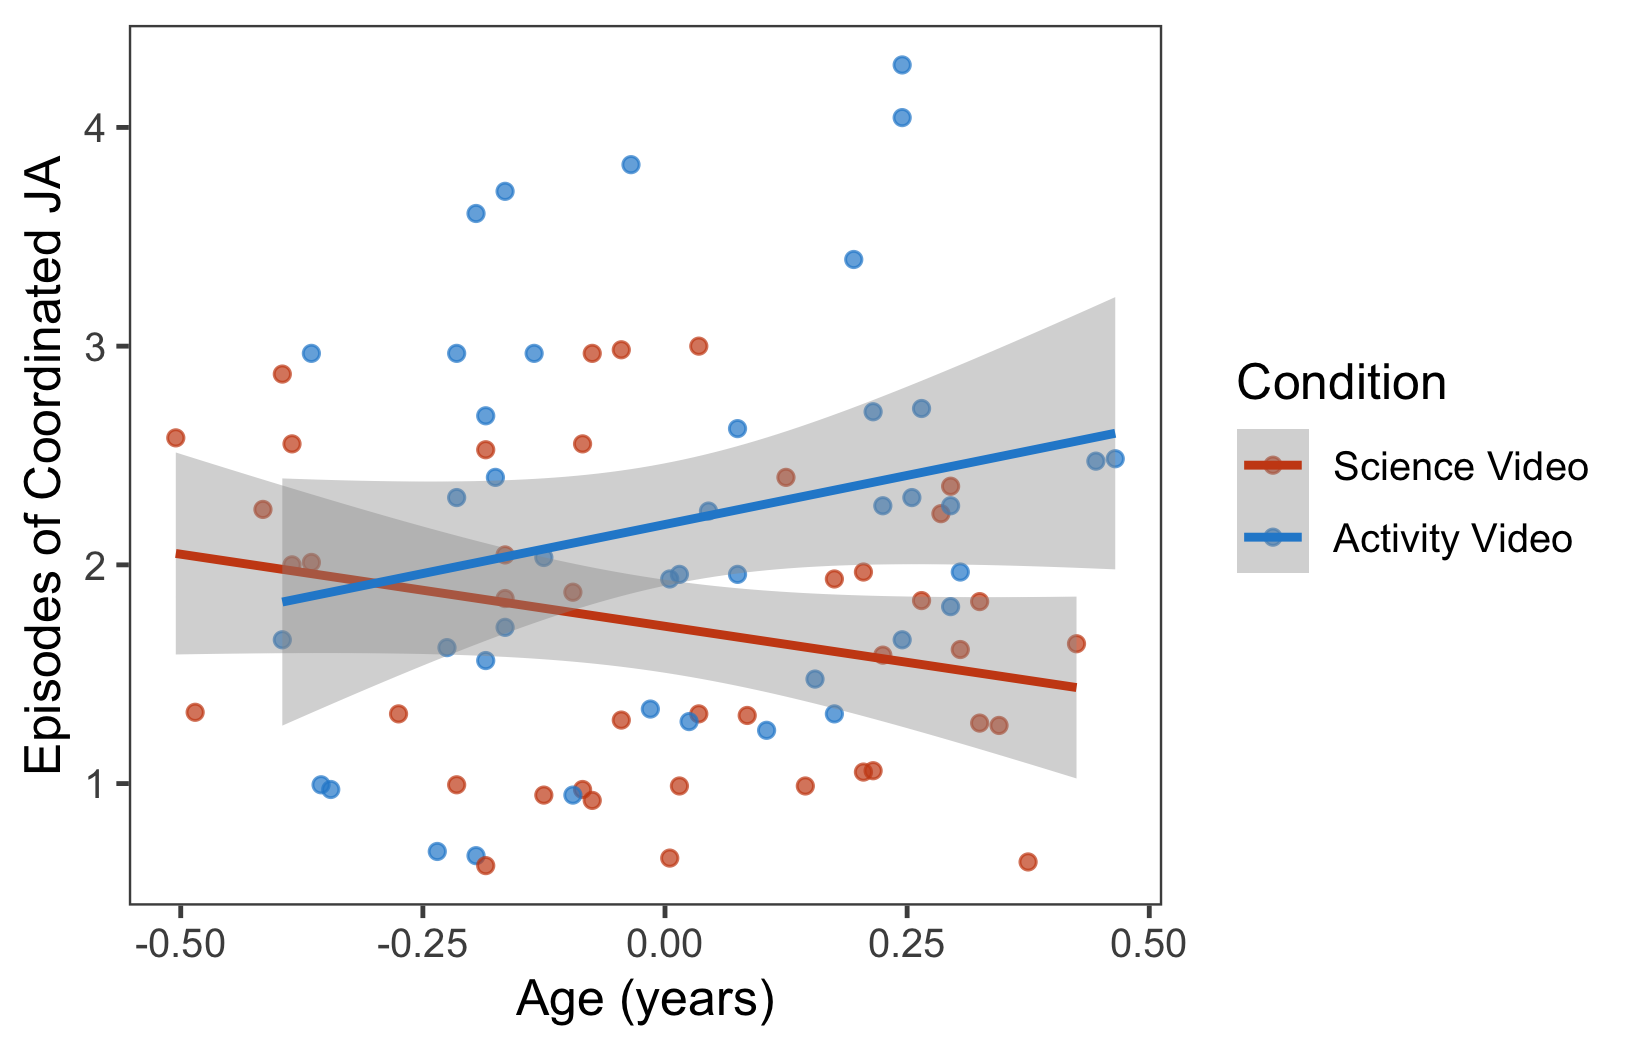
\includegraphics{figs/e2ja-coord-1} 

}

\caption{The number of episodes of coordinated JA by condition and age in Experiment 2.}\label{fig:e2ja-coord}
\end{figure}

\hypertarget{general-discussion}{%
\section{General Discussion}\label{general-discussion}}

We were interested in how digital parenting advice alters parents' interactions with their children.
We specifically set out to test whether activity suggestions led to higher-quality play, a presupposition of many early parenting interventions.
Our experiments explored this question by randomly assigning parents to different advice conditions and then observing their behavior in short free-play sessions, with quality of play assessed through measures of parent language and joint attention.
In two experiments, we found that activity videos increased the rate of parents' bids for joint attention as compared with no video (Experiment 1) and a comparable science video (Experiment 2).
In some cases---especially in older children---these bids were successful in increasing engagement.
We also observed differences in parents' talk that were broadly similar across both experiments, with a greater quantity of language but a similar breadth of vocabulary (leading to lower measures of lexical diversity).
Exploratory corpus analysis identified the words most characteristic of the activity videos as being related to requests (e.g., \enquote{give}, \enquote{put}, \enquote{take}) whereas control conditions featured more invitational words (e.g., \enquote{say}, \enquote{let}, \enquote{like}), often asking about animal noises (\enquote{What does the X say?}).

The short, activity-oriented parenting messages we used encouraged parents to make more attempts---both verbal and non-verbal---to engage their child, supporting their use as a component of interventions.
Why were they successful?
When parents are asked to play with their children in the presence of new toys, they may choose to follow their child's lead and engage in free play.
While free play is positive, it nevertheless results in less scaffolded activity than when parents are given a goal that suggests a repertoire of ways to guide their child.
Parents may also persist in providing opportunities for their child to complete the activity, leading to more repetitive language but also more offers of engagement.

Our study has a number of limitations related to design and sample, each of which suggests possible future directions.
First, our design was intentionally short and minimal; future studies should investigate whether changes in parents' speech and attempts to engage their children could persist across a longer timespan (perhaps with a broader set of activities being provisioned).
A longer-term study would also address whether consistent increases in parent bids would lead children to respond by engaging more with their parent.
Second, our design assumes that parents have access to the materials needed to complete the suggested activities; this assumption may be unrealistic for any parent, but especially for the parents who are most likely to be targeted for early parenting interventions.
Providing materials may be critical for the success of activity suggestions.
Finally, our sample is a convenience sample drawn from a museum, but it skews towards higher socio-economic status households as well as those families who are well-disposed towards visiting a museum (perhaps because they value education) and are interested in participating in research.
A key goal for future research is to assess the generality of these findings across populations.

In sum, the results of this study show that digital parenting videos recommending play activities can lead to short-term increases in parents' attempts to engage their young children, both verbally and non-verbally.

\hypertarget{acknowledgements}{%
\section{Acknowledgements}\label{acknowledgements}}

This work was supported by a gift and a contract from Kinedu, Inc.~to the Language and Cognition Lab.
Thanks to Samaher Radwan and Megan Merrick for behavioral coding of the videos, and to members of the Language and Cognition Lab at Stanford for helpful discussion.

\newpage

\hypertarget{references}{%
\section{References}\label{references}}

\begingroup
\setlength{\parindent}{-0.5in}
\setlength{\leftskip}{0.5in}

\hypertarget{refs}{}
\leavevmode\hypertarget{ref-Baldwin1991}{}%
Baldwin, D. (1991). Infants' contribution to the achievement of joint reference. \emph{Child Development}, \emph{62}, 875--890.

\leavevmode\hypertarget{ref-Bigelow2004}{}%
Bigelow, A. E., MacLean, K., \& Proctor, J. (2004). The role of joint attention in the development of infants' play with objects. \emph{Developmental Science}, \emph{7}, 518--526.

\leavevmode\hypertarget{ref-Breitenstein2016}{}%
Breitenstein, S. M., Fogg, L., Ocampo, E. V., Acosta, D. I., \& Gross, D. (2016). Parent use and efficacy of a self-administered, tablet-based parent training intervention: A randomized controlled trial. \emph{JMIR mHealth and uHealth}, \emph{4}(2), e36. \url{http://doi.org/10.2196/mhealth.5202}

\leavevmode\hypertarget{ref-Breitenstein2014}{}%
Breitenstein, S. M., Gross, D., \& Christophersen, R. (2014). Digital delivery methods of parenting training interventions: A systematic review. \emph{Worldviews on Evidence-Based Nursing}, \emph{11}, 168--176.

\leavevmode\hypertarget{ref-Cartmill2013}{}%
Cartmill, E. A., Armstrong, B. F., Gleitman, L. R., Goldin-Meadow, S., Medina, T. N., \& Trueswell, J. C. (2013). Quality of early parent input predicts child vocabulary 3 years later. \emph{Proceedings of the National Academy of Sciences}, \emph{110}(28), 11278--11283. \url{http://doi.org/10.1073/pnas.1309518110}

\leavevmode\hypertarget{ref-Jamaica2014}{}%
Gertler, P., Heckman, J., Pinto, R., Zanolini, A., Vermeersch, C., Walker, S., \ldots{} Grantham-McGregor, S. (2014). Labor market returns to an early childhood stimulation intervention in jamaica. \emph{Science}, \emph{344}(6187), 998--1001. \url{http://doi.org/10.1126/science.1251178}

\leavevmode\hypertarget{ref-rstanarm}{}%
Goodrich, B., Gabry, J., Ali, I., \& Brilleman, S. (2018). Rstanarm: Bayesian applied regression modeling via Stan. Retrieved from \url{http://mc-stan.org/}

\leavevmode\hypertarget{ref-Hart1995}{}%
Hart, B., \& Risley, T. R. (1995). \emph{Meaningful differences in the everyday experience of young american children}. Baltimore, MD: Brookes.

\leavevmode\hypertarget{ref-Heckman2006}{}%
Heckman, J. J. (2006). Skill formation and the economics of investing in disadvantaged children. \emph{Science}, \emph{312}(5782), 1900--1902. \url{http://doi.org/10.1126/science.1128898}

\leavevmode\hypertarget{ref-Hembacher2020}{}%
Hembacher, E., \& Frank, M. C. (2020). The early parenting attitudes questionnaire: Measuring intuitive theories of parenting and child development. \emph{Collabra: Psychology}, \emph{6}(1). \url{http://doi.org/10.31234/osf.io/hxk3d}

\leavevmode\hypertarget{ref-HirshPasek2015}{}%
Hirsh-Pasek, K., Adamson, L. B., Bakeman, R., Owen, M. T., Golinkoff, R. M., Pace, A., \ldots{} Suma, K. (2015). The contribution of early communication quality to low-income children's language success. \emph{Psychological Science}, \emph{26}(7), 1071--1083. \url{http://doi.org/10.1177/0956797615581493}

\leavevmode\hypertarget{ref-Kruschke2014}{}%
Kruschke, J. (2014). \emph{Doing bayesian data analysis: A tutorial with r, jags, and stan}. Academic Press.

\leavevmode\hypertarget{ref-Leung2018}{}%
Leung, C. Y., Hernandez, M. W., \& Suskind, D. L. (2018). Enriching home language environment among families from low-ses backgrounds: A randomized controlled trial of a home visiting curriculum. \emph{Early Childhood Research Quarterly}. \url{http://doi.org/https://doi.org/10.1016/j.ecresq.2018.12.005}

\leavevmode\hypertarget{ref-Makowski2019}{}%
Makowski, D., Ben-Shachar, M. S., Chen, S. H. A., \& Lüdecke, D. (2019a). Indices of effect existence and significance in the bayesian framework. \emph{Frontiers in Psychology}, \emph{10}, 2767. \url{http://doi.org/10.3389/fpsyg.2019.02767}

\leavevmode\hypertarget{ref-bayestestR}{}%
Makowski, D., Ben-Shachar, M. S., \& Lüdecke, D. (2019b). BayestestR: Describing effects and their uncertainty, existence and significance within the bayesian framework. \emph{Journal of Open Source Software}, \emph{4}(40), 1541. \url{http://doi.org/10.21105/joss.01541}

\leavevmode\hypertarget{ref-Malvern2004}{}%
Malvern, D., Richards, B. J., Chipere, N., \& Durán, P. (2004). \emph{Lexical diversity and language development}. Palgrave Macmillan.

\leavevmode\hypertarget{ref-Marchman2008}{}%
Marchman, V. A., \& Fernald, A. (2008). Speed of word recognition and vocabulary knowledge in infancy predict cognitive and language outcomes in later childhood. \emph{Developmental Science}, \emph{11}, F9--F16.

\leavevmode\hypertarget{ref-McCarthy2010}{}%
McCarthy, P. M., \& Jarvis, S. (2010). MTLD, vocd-d, and hd-d: A validation study of sophisticated approaches to lexical diversity assessment. \emph{Behavior Research Methods}, \emph{42}(2), 381--392.

\leavevmode\hypertarget{ref-McElreath2018}{}%
McElreath, R. (2018). \emph{Statistical rethinking: A bayesian course with examples in r and stan}. Chapman; Hall/CRC.

\leavevmode\hypertarget{ref-Schwab2016}{}%
Schwab, J. F., \& Lew-Williams, C. (2016). Language learning, socioeconomic status, and child-directed speech. \emph{WIREs Cognitive Science}, \emph{7}, 264--275. \url{http://doi.org/10.1002/wcs.1393}

\leavevmode\hypertarget{ref-PerryPreschool2004}{}%
Schweinhart, L. J., Montie, J., Xiang, Z., Barnett, W. S., Belfield, C. R., \& Nores, M. (2004). \emph{Lifetime effects: The highscope perry preschool study through age 40}. Ypsilanti, MI: HighScope Press.

\leavevmode\hypertarget{ref-datavyu}{}%
Team, D. (2014). Datavyu: A video coding tool. \emph{Databrary Project}. Retrieved from \url{http://datavyu.org}

\leavevmode\hypertarget{ref-Weisberg2013}{}%
Weisberg, D. S., Hirsh-Pasek, K., \& Golinkoff, R. M. (2013). Guided play: Where curricular goals meet a playful pedagogy. \emph{Mind, Brain, and Education}, \emph{7}, 104--112.

\leavevmode\hypertarget{ref-Wood1976}{}%
Wood, D., Bruner, J. S., \& Ross, G. (1976). The role of tutoring in problem solving. \emph{Journal of Child Psychology and Psychiatry}, \emph{17}, 89--100.

\leavevmode\hypertarget{ref-Baldwin1991}{}%
Baldwin, D. (1991). Infants' contribution to the achievement of joint reference. \emph{Child Development}, \emph{62}, 875--890.

\leavevmode\hypertarget{ref-Bigelow2004}{}%
Bigelow, A. E., MacLean, K., \& Proctor, J. (2004). The role of joint attention in the development of infants' play with objects. \emph{Developmental Science}, \emph{7}, 518--526.

\leavevmode\hypertarget{ref-Breitenstein2016}{}%
Breitenstein, S. M., Fogg, L., Ocampo, E. V., Acosta, D. I., \& Gross, D. (2016). Parent use and efficacy of a self-administered, tablet-based parent training intervention: A randomized controlled trial. \emph{JMIR mHealth and uHealth}, \emph{4}(2), e36. \url{http://doi.org/10.2196/mhealth.5202}

\leavevmode\hypertarget{ref-Breitenstein2014}{}%
Breitenstein, S. M., Gross, D., \& Christophersen, R. (2014). Digital delivery methods of parenting training interventions: A systematic review. \emph{Worldviews on Evidence-Based Nursing}, \emph{11}, 168--176.

\leavevmode\hypertarget{ref-Cartmill2013}{}%
Cartmill, E. A., Armstrong, B. F., Gleitman, L. R., Goldin-Meadow, S., Medina, T. N., \& Trueswell, J. C. (2013). Quality of early parent input predicts child vocabulary 3 years later. \emph{Proceedings of the National Academy of Sciences}, \emph{110}(28), 11278--11283. \url{http://doi.org/10.1073/pnas.1309518110}

\leavevmode\hypertarget{ref-Jamaica2014}{}%
Gertler, P., Heckman, J., Pinto, R., Zanolini, A., Vermeersch, C., Walker, S., \ldots{} Grantham-McGregor, S. (2014). Labor market returns to an early childhood stimulation intervention in jamaica. \emph{Science}, \emph{344}(6187), 998--1001. \url{http://doi.org/10.1126/science.1251178}

\leavevmode\hypertarget{ref-rstanarm}{}%
Goodrich, B., Gabry, J., Ali, I., \& Brilleman, S. (2018). Rstanarm: Bayesian applied regression modeling via Stan. Retrieved from \url{http://mc-stan.org/}

\leavevmode\hypertarget{ref-Hart1995}{}%
Hart, B., \& Risley, T. R. (1995). \emph{Meaningful differences in the everyday experience of young american children}. Baltimore, MD: Brookes.

\leavevmode\hypertarget{ref-Heckman2006}{}%
Heckman, J. J. (2006). Skill formation and the economics of investing in disadvantaged children. \emph{Science}, \emph{312}(5782), 1900--1902. \url{http://doi.org/10.1126/science.1128898}

\leavevmode\hypertarget{ref-Hembacher2020}{}%
Hembacher, E., \& Frank, M. C. (2020). The early parenting attitudes questionnaire: Measuring intuitive theories of parenting and child development. \emph{Collabra: Psychology}, \emph{6}(1). \url{http://doi.org/10.31234/osf.io/hxk3d}

\leavevmode\hypertarget{ref-HirshPasek2015}{}%
Hirsh-Pasek, K., Adamson, L. B., Bakeman, R., Owen, M. T., Golinkoff, R. M., Pace, A., \ldots{} Suma, K. (2015). The contribution of early communication quality to low-income children's language success. \emph{Psychological Science}, \emph{26}(7), 1071--1083. \url{http://doi.org/10.1177/0956797615581493}

\leavevmode\hypertarget{ref-Kruschke2014}{}%
Kruschke, J. (2014). \emph{Doing bayesian data analysis: A tutorial with r, jags, and stan}. Academic Press.

\leavevmode\hypertarget{ref-Leung2018}{}%
Leung, C. Y., Hernandez, M. W., \& Suskind, D. L. (2018). Enriching home language environment among families from low-ses backgrounds: A randomized controlled trial of a home visiting curriculum. \emph{Early Childhood Research Quarterly}. \url{http://doi.org/https://doi.org/10.1016/j.ecresq.2018.12.005}

\leavevmode\hypertarget{ref-Makowski2019}{}%
Makowski, D., Ben-Shachar, M. S., Chen, S. H. A., \& Lüdecke, D. (2019a). Indices of effect existence and significance in the bayesian framework. \emph{Frontiers in Psychology}, \emph{10}, 2767. \url{http://doi.org/10.3389/fpsyg.2019.02767}

\leavevmode\hypertarget{ref-bayestestR}{}%
Makowski, D., Ben-Shachar, M. S., \& Lüdecke, D. (2019b). BayestestR: Describing effects and their uncertainty, existence and significance within the bayesian framework. \emph{Journal of Open Source Software}, \emph{4}(40), 1541. \url{http://doi.org/10.21105/joss.01541}

\leavevmode\hypertarget{ref-Malvern2004}{}%
Malvern, D., Richards, B. J., Chipere, N., \& Durán, P. (2004). \emph{Lexical diversity and language development}. Palgrave Macmillan.

\leavevmode\hypertarget{ref-Marchman2008}{}%
Marchman, V. A., \& Fernald, A. (2008). Speed of word recognition and vocabulary knowledge in infancy predict cognitive and language outcomes in later childhood. \emph{Developmental Science}, \emph{11}, F9--F16.

\leavevmode\hypertarget{ref-McCarthy2010}{}%
McCarthy, P. M., \& Jarvis, S. (2010). MTLD, vocd-d, and hd-d: A validation study of sophisticated approaches to lexical diversity assessment. \emph{Behavior Research Methods}, \emph{42}(2), 381--392.

\leavevmode\hypertarget{ref-McElreath2018}{}%
McElreath, R. (2018). \emph{Statistical rethinking: A bayesian course with examples in r and stan}. Chapman; Hall/CRC.

\leavevmode\hypertarget{ref-Schwab2016}{}%
Schwab, J. F., \& Lew-Williams, C. (2016). Language learning, socioeconomic status, and child-directed speech. \emph{WIREs Cognitive Science}, \emph{7}, 264--275. \url{http://doi.org/10.1002/wcs.1393}

\leavevmode\hypertarget{ref-PerryPreschool2004}{}%
Schweinhart, L. J., Montie, J., Xiang, Z., Barnett, W. S., Belfield, C. R., \& Nores, M. (2004). \emph{Lifetime effects: The highscope perry preschool study through age 40}. Ypsilanti, MI: HighScope Press.

\leavevmode\hypertarget{ref-datavyu}{}%
Team, D. (2014). Datavyu: A video coding tool. \emph{Databrary Project}. Retrieved from \url{http://datavyu.org}

\leavevmode\hypertarget{ref-Weisberg2013}{}%
Weisberg, D. S., Hirsh-Pasek, K., \& Golinkoff, R. M. (2013). Guided play: Where curricular goals meet a playful pedagogy. \emph{Mind, Brain, and Education}, \emph{7}, 104--112.

\leavevmode\hypertarget{ref-Wood1976}{}%
Wood, D., Bruner, J. S., \& Ross, G. (1976). The role of tutoring in problem solving. \emph{Journal of Child Psychology and Psychiatry}, \emph{17}, 89--100.

\endgroup

\clearpage
\makeatletter
\efloat@restorefloats
\makeatother


\begin{appendix}
\section{}
\hypertarget{experiment-1-activities}{%
\subsection{Experiment 1 Activities}\label{experiment-1-activities}}

\hypertarget{video-a-6-11.9-months-pick-it-up}{%
\subsubsection{Video A (6-11.9 months) ``Pick it
up''}\label{video-a-6-11.9-months-pick-it-up}}

Parents are told to encourage their child to pick up and drop individual
objects. They are also encouraged to place toys on a small cloth and
show the child that they can drag the cloth towards them to reach the
toys.

Props: cloth, plastic horse, plastic sheep, plastic elephant, toy car

\hypertarget{video-b-6-11.9-months-animal-sounds}{%
\subsubsection{Video B (6-11.9 months) ``Animal
sounds''}\label{video-b-6-11.9-months-animal-sounds}}

Parents are told to call different animals and imitate different sounds
the animals make. They are also encouraged to observe which animal the
child prefers.

Props: plastic sheep, plastic horse, plastic frog, plastic cow, bowls

\hypertarget{video-c-12-17.9-months-give-me-the-toy}{%
\subsubsection{Video C (12-17.9 months) ``Give me the
toy''}\label{video-c-12-17.9-months-give-me-the-toy}}

Parents are told to ask their child to hand over individual toys. They
are also encouraged to praise the child after they give them the toys,
and repeat the process until the child follows the verbal instructions.

Props: toy boat, plastic frog, plastic elephant, toy bus

\hypertarget{video-d-12-17.9-months-classifying-my-toys}{%
\subsubsection{Video D (12-17.9 months) ``Classifying my
toys''}\label{video-d-12-17.9-months-classifying-my-toys}}

Parents are told to place toys of different sizes (big or small) in two
hoops. They are also encouraged to ask their child to distinguish
between two objects and identify which one is larger.

Props: two yellow and green rings, big car, small car, big horse, small
horse

\hypertarget{video-e-18-23.9-months-my-toys}{%
\subsubsection{Video E (18-23.9 months) ``My
toys''}\label{video-e-18-23.9-months-my-toys}}

Parents are told to show the child toys of the same shape but different
sizes, to place one of the objects in a basket and to ask the child to
take out the object. They are also encouraged to ask their child if the
object is bigger or smaller compared to its pair.

Props: two buckets, big car, small car, big horse, small horse

\hypertarget{video-f-18-23.9-months-the-orchestra}{%
\subsubsection{Video F (18-23.9 months) ``The
orchestra''}\label{video-f-18-23.9-months-the-orchestra}}

Parents are told to give their child a musical instrument to play. They
are also encouraged to play a song and see if the child follows the
rhythm.

Props: maracas, drum, tambourine, clapper

\hypertarget{experiment-2-activities}{%
\subsection{Experiment 2 Activities}\label{experiment-2-activities}}

\hypertarget{video-a-12-17.9-months-give-me-the-toy}{%
\subsubsection{Video A (12-17.9 months) ``Give me the
toy''}\label{video-a-12-17.9-months-give-me-the-toy}}

Parents are told to ask their child to hand over individual toys. They
are also encouraged to praise the child after they give them the toys,
and repeat the process until the child follows the verbal instructions.

Props: plastic pig, plastic horse, plastic dog, plastic cat, plastic cow

\hypertarget{video-b-12-17.9-months-classifying-my-toys}{%
\subsubsection{Video B (12-17.9 months) ``Classifying my
toys''}\label{video-b-12-17.9-months-classifying-my-toys}}

Parents are told to place toys of different sizes (big or small) in two
hoops. They are also encouraged to ask their child to distinguish
between two objects and identify which one is larger.

Props: two yellow and green rings, big car, small car, big horse, small
horse

\hypertarget{video-c-12-17.9-months-geometric-shapes-jigsaw-puzzle}{%
\subsubsection{Video C (12-17.9 months) ``Geometric shapes jigsaw
puzzle''}\label{video-c-12-17.9-months-geometric-shapes-jigsaw-puzzle}}

Parents are told to encourage their child to name different shapes on a
jigsaw puzzle. Then they are told to undo the puzzle and invite the
child to complete the puzzle.

Props: A jigsaw puzzle of geometric shapes

\hypertarget{video-d-18-23.9-months-my-toys}{%
\subsubsection{Video D (18-23.9 months) ``My
toys''}\label{video-d-18-23.9-months-my-toys}}

Parents are told to show the child toys of the same shape but different
sizes, to place one of the objects in a basket and to ask the child to
take out the object. They are also encouraged to ask their child if the
object is bigger or smaller compared to its pair.

Props: two buckets, big car, small car, big horse, small horse

\hypertarget{video-e-18-23.9-months-the-orchestra}{%
\subsubsection{Video E (18-23.9 months) ``The
orchestra''}\label{video-e-18-23.9-months-the-orchestra}}

Parents are told to give their child a musical instrument to play. They
are also encouraged to play a song and see if the child follows the
rhythm.

Props: maracas, drum, tambourine, clapper

\hypertarget{video-f-18-23.9-months-my-yellow-toys}{%
\subsubsection{Video F (18-23.9 months) ``My yellow
toys''}\label{video-f-18-23.9-months-my-yellow-toys}}

Parents are told to show their child yellow toys and to ask, ``What
color are they?'' They are also told to give the child toys of different
colors, to ask them to only play with the yellow ones, and to praise the
child after they do so.

Props: blue car, yellow car, yellow block, red block, blue block, green
block
\end{appendix}

\end{document}
